\documentclass[times, utf8, seminar, english]{fer}
\usepackage{booktabs}
\usepackage{epigraph}
\usepackage{mathtools, amsmath,amsfonts,amssymb, amsthm}
\usepackage{hyperref}
\usepackage{fancybox}
\usepackage{graphicx}
\graphicspath{ {img/} }
\usepackage{etoolbox}

\makeatletter
\patchcmd{\chapter}{\if@openright\cleardoublepage\else\clearpage\fi}{}{}{}
\makeatother
\usepackage{minted}
\begin{document}
\theoremstyle{definition}
\newtheorem{definition}{Definition}[section]
\title{iproute2 and iptables packet}
\author{Neven Miculinic}

\maketitle
\tableofcontents

\chapter{Introduction}

Networking is one of the most important topic in everyday computer use. Almost every meaningful action we do in digital forencis, sooner or later involves networkings. Whether it's simply performing backups, viewing facebook messages, sending emails, or accessing databases and utilizing VPN/SSH.
As in any complex system, one surely describing networking, many things may go wrong and multiple attacks are possible. For the computer forensics purpose, this essay describes bacis linux networking primities, from the time network packet enters the machine, reaches local process, and exits the machine.

It describes two tools consisting used most commonly in Linux networking. First is iptables, part of Netfilter project. Netfilter~\cite{netfilte6:online} is a framework providing various kernel hooks within network stack allowing user to modify and alter network packages. IPtables is their most commonly used utility. It shall be decribed in more detail in following chapters.

Iproute~\cite{shemming47:online} is a collection of userspace utilities for controlling and monitoring various aspects of networking in the Linux kernel, including routing, network interfaces, tunnels, traffic control, and network-related device drivers. In this essay the focus in only on routing, and just a brief introduction and basic/most common commands.

\chapter{iptables}
This chapter desvribes packet path through various iptables tables and chains. The rest of the chapter is dedicated for explaining basic ip tables concept, with next chapter showing various application.
Visual overview can be seen in figure~\ref{fig:iptables_traverse}.

\begin{figure}
    \centering
    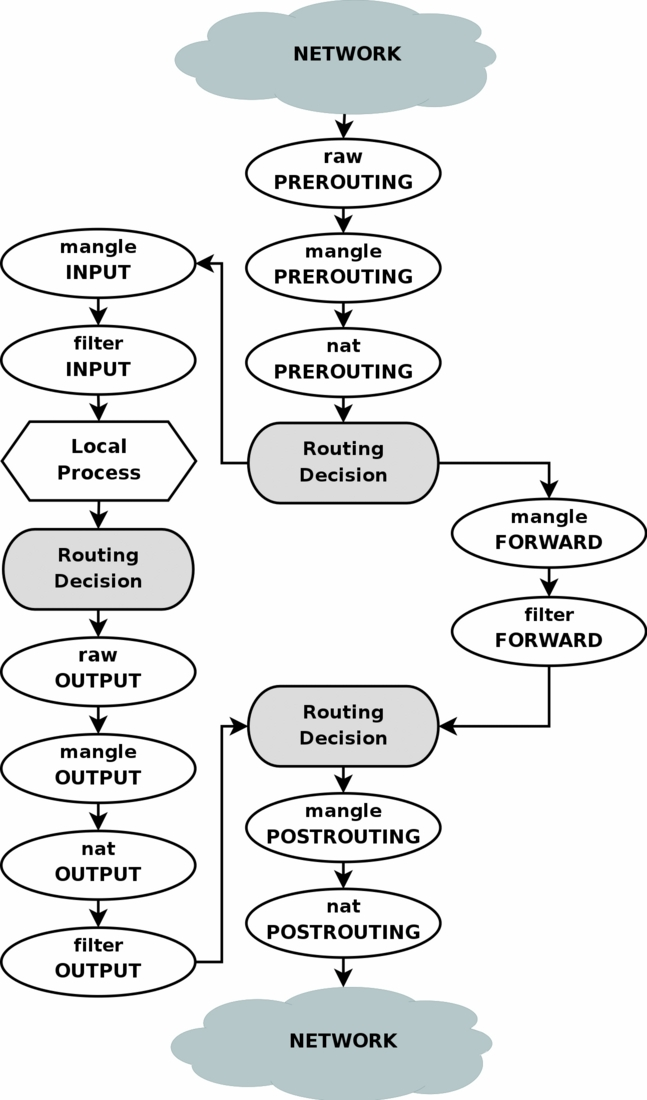
\includegraphics[width=0.8\textwidth]{tables_traverse}
    \caption{Overview of iptables. The lowercase word on top is the table and the upper case word below is the chain. Source~\cite{Iptables99:online}}
    \label{fig:iptables_traverse}
\end{figure}

\section{Rule}
    Iptables have various rule, when matches their target is executed. They function as if-then construct. The most common rule 'ifs' are source/destination address, protocol and/or interface. They can be combined with and/or clauses. Furthermore any valid BPF~\cite{BPFthefo6:online} bytecode can be rule 'if'

    The most common rule targets are ACCEPT, DROP, REJECT ones which perform packet filtering. In NAT table, common ones are DNAT, SNAT and MASQUERADE which perform IP:port NATing. They shall be described in more detail in later sections. Other common rule targets are LOG and jump to another chain.

\section{Chain}
    Chain is a list of rules which are matched in order. Rule can be terminal (most of them) or nonterminal (e.g. LOG,  ULOG). Upon reaching the terminal rule (e.g. DROP) chain has reached its end. Chain can have it's default policy (e.g. DROP for table filter in INPUT chain).
    There are two types of chains -- system (PREROURING, INPUT, FORWARD, OUTPUT, POSTROUTING) and user defined chains.
    User defined chains server se target jump within the same table (e.g. jump to user defined chain).
    They are created with \verb|iptables -N <chain_name> -t <table name [filter default]>|.
    Chain traversal is depicted in figure~\ref{fig:iptables_subtraverse}. System chains are:

    \begin{itemize}
        \item PREROURING -- Packet arriving in the kernel before any routing
        \item INPUT -- Packet is destined for the local process
        \item FORWARD -- Packet isn't destined for the local process
        \item OUTPUT -- Packet originated from local process
        \item POSTROUTING -- Packet departing from the machine after all routing takes place
    \end{itemize}
    Refer to figure~\ref{fig:iptables_traverse} for their interaction.

    \begin{figure}
        \centering
        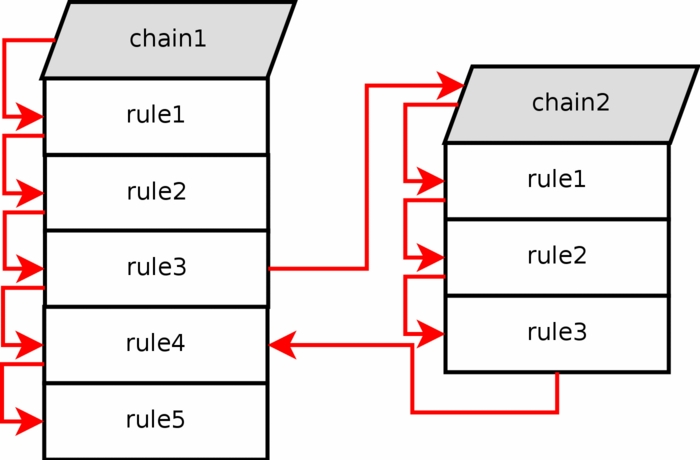
\includegraphics[width=0.8\textwidth]{table_subtraverse}
        \caption{Table chain subtraverstion. Source~\cite{Iptables99:online}}
        \label{fig:iptables_subtraverse}
    \end{figure}
\section{Tables}
    Tables are bread and butter of this package. Each table defines specific hooks in the kernel for various system chains. They are associated with specific chain (that is NAT table in PREROURING and POSTROUTING are different). Each table is composed of multipe chains, what system defined ones, what user defined chains.
    There are 5 tables:
    \begin{itemize}
        \item raw -- applied before any connection tracking takes place
        \item mangle -- Mostly used for quality-of-service (QoS) header bit setting
        \item filter -- packet filtering (DROP, ACCEPT and REJECT tagets)
        \item nat -- NATing packages (DNAT, SNAT, MASQUERADE)
        \item security --
    \end{itemize}
    Refer to link~\cite{Iptables27:online} for more detail.

    \section{Extensions}
    Iptables offers multiple modules you can use.
    You can view all installed modules by \texttt{ls -l /lib/iptables} and iptables will load all required modules dynamically.


\section{Routing tables}
\section{Network namespaces}


\chapter{Example usecases}
pass
\section{OpenVPN on Google cloud platform}
pass
\section{Isolating process in its own network namespace}

\section{Disabling internet access for specific device at specific time}

For example you might have a really smart teen adicted to the internet.
And you'd like disabling his internet access at the router level at certain times, while keeping rest functioning.
It can be simly done with one iptables command and few extra modules

\begin{minted}{bash}
iptables -A PREROURING -m mac --mac-source 00:0F:EA:91:04:08 \
    -m time --timestart 9:00 --timestop 18:00 -j ACCEPT
iptables -A PREROURING -m mac --mac-source 00:0F:EA:91:04:08 \
    -j DROP
\end{minted}

This is more efficient than IP filtering since you're probably running DHCP on your network dynamically assigning IP addresses.
Nevertheless, it's easy for attacker (your teen) to figure out his MAC address is filterer, and to spoof it.
Yet, hopefully by the time he figures it out, he'll already be a functional adult.

\bibliography{refs}
\bibliographystyle{fer}

\end{document}
